\documentclass{standalone}
\usepackage{tikz}
\usetikzlibrary{quotes,angles}
\begin{document}
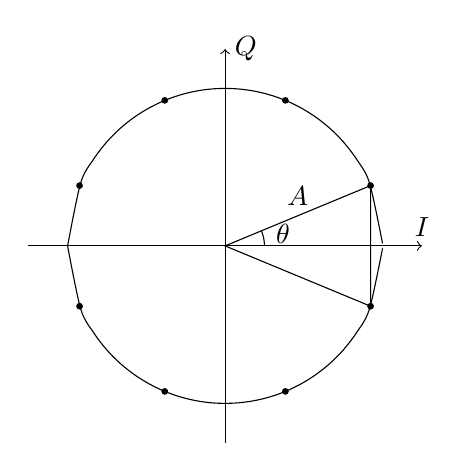
\begin{tikzpicture}[scale=2]
    \draw[->](-1.25,0)--(1.25,0)node[above]{$I$};
    \draw[->](0,-1.25)--(0,1.25)node[right]{$Q$};

    \draw[smooth, domain=-1:1]plot(\x,{(1-(\x)^2)^0.5});
    \draw[smooth, domain=-1:1]plot(\x,{-(1-(\x)^2)^0.5});
    \filldraw[black](0.924,0.383)circle(0.5pt);
    \filldraw[black](0.924,-0.383)circle(0.5pt);
    \filldraw[black](-0.924,0.383)circle(0.5pt);
    \filldraw[black](-0.924,-0.383)circle(0.5pt);
    \filldraw[black](0.383,0.924)circle(0.5pt);
    \filldraw[black](0.383,-0.924)circle(0.5pt);
    \filldraw[black](-0.383,0.924)circle(0.5pt);
    \filldraw[black](-0.383,-0.924)circle(0.5pt);

    \coordinate(o)at(0,0);
    \coordinate(a1)at(0.924,0.383);
    \coordinate(a2)at(1,0);
    \pic[draw, "$\theta$", angle eccentricity=1.5,radius=0.6cm]{angle=a2--o--a1};
    \draw[-](0.924,0.383)--(0,0)node[midway, above]{$A$}--(0.924,-0.383)--(0.924,0.383);
\end{tikzpicture}
\end{document}